%%%%%%%%%%%%%%%%%%%%%%%%%%%%%%%%%%%%%%%%%%%%%%%%%%%%%%%
%% Bachelor's & Master's Thesis Template             %%
%% Copyleft by Artur M. Brodzki & Piotr Woźniak      %%
%% Faculty of Electronics and Information Technology %%
%% Warsaw University of Technology, 2019-2020        %%
%%%%%%%%%%%%%%%%%%%%%%%%%%%%%%%%%%%%%%%%%%%%%%%%%%%%%%%

\documentclass[
    left=2.5cm,         % Sadly, generic margin parameter
    right=2.5cm,        % doesnt't work, as it is
    top=2.5cm,          % superseded by more specific
    bottom=3cm,         % left...bottom parameters.
    bindingoffset=6mm,  % Optional binding offset.
    nohyphenation=false % You may turn off hyphenation, if don't like.
]{eiti/eiti-thesis}

\langpol % Dla języka angielskiego mamy \langeng
\usepackage{graphicx}
%\usepackage{biblatex}
\graphicspath{{img/}} 
\usepackage{float} % Katalog z obrazkami.
% \addbibresource{bibliografia.bib} % Plik .bib z bibliografią
\usepackage{graphicx} 
\usepackage{listings}
\usepackage{xcolor}
\usepackage{enumitem}

\usepackage[utf8]{inputenc}
\usepackage[T1]{fontenc}
\usepackage[polish]{babel}
\usepackage{csquotes}

\usepackage[backend=biber]{biblatex}


\addbibresource{bibliografia.bib}
	


\begin{document}

%--------------------------------------
% Strona tytułowa
%--------------------------------------
\MasterThesis % Dla pracy inżynierskiej mamy \EngineerThesis
\instytut{Informatyki}
\kierunek{Informatyka}
\specjalnosc{Informatyka w multimediach}
\title{
	Zastosowanie głębokich sieci neuronowych\\ w detekcji chorób roślin
}
\engtitle{ % Tytuł po angielsku do angielskiego streszczenia
   Application of Deep Neural Networks in Plant Disease Detection
}
\author{Jakub Piotr Kostrzewa}
\album{}
\promotor{Prof. Przemysław Rokita}
\date{\the\year}
\maketitle

%--------------------------------------
% Streszczenie po polsku
%--------------------------------------
\cleardoublepage % Zaczynamy od nieparzystej strony
\streszczenie Celem pracy magisterskiej było zbadanie wybranych modeli głębokiego uczenia w zadaniu klasyfikacji wieloklasowej obrazów roślin oraz określenie wpływu ilości i jakości danych treningowych na uzyskiwane wyniki. W ramach badania przeanalizowano dziesięć modeli należących do pięciu rodzin architektur: ResNet, Vision Transformer(ViT), DenseNet, MobileNet, EfficientNet.

 Przeprowadzono dwa eksperymenty w ramach, których modele były szkolone na różnych zbiorach danych, z użyciem techniki transfer learning. Wszystkie modele były wstępnie przetrenowane na tym samym zbiorze. W ramach pierwszego eksperymentu zbadano wpływ ograniczenia ilości danych na jakość klasyfikacji, a w drugim wpływ jakości zbioru treningowego. Jako pierwotny zbiór danych został wykorzystany zbiór PlantVillage-Dataset. Do każdego z eksperymentów przygotowano oddzielne zbiory. Do analizy wyników wykorzystano miarę Macro-F1 Score.
 
 Uzyskane Wyniki wskazały, że większość analizowanych modeli osiąga wysokie wartości miary Macro-F1 w tym zadaniu. Jedynym wyjątkiem były modele DenseNet, które osiągnęły najgorsze wyniki w całym zestawieniu, zdecydowanie niższe od reszty.  Modele oparte o transformery nie uzyskały przewagi nad modelami CNN. Najlepszymi modelami okazały się modele z rodzin MobileNet i EfficientNet. Wyniki wskazują na potencjał zbadanych modeli do praktycznego wykorzystania.

\slowakluczowe uczenie głębokie, sieci neuronowe, klasyfikacja danych, choroby roślin

%--------------------------------------
% Streszczenie po angielsku
%--------------------------------------
\newpage
\abstract The aim of this master's thesis was to investigate selected deep learning models for multiclass classification of plant images and determine the impact of the quantity and quality of training data on the obtained results. The study analyzed ten models belonging to five architecture families: ResNet, Vision Transformer (ViT), DenseNet, MobileNet, and EfficientNet.

Two experiments were conducted in which the models were trained on different datasets using transfer learning. All models were pre-trained on the same dataset. The first experiment examined the impact of data limitation on classification quality, while the second examined the impact of training set quality. The PlantVillage-Dataset was used as the initial dataset. Separate datasets were prepared for each experiment. The Macro-F1 Score was used to analyze the results.

The obtained results indicated that most of the analyzed models achieved high Macro-F1 scores in this task. The only exception were the DenseNet models, which achieved the worst results in the entire comparison, significantly lower than the rest. Transformer-based models did not demonstrate an advantage over CNN models. The best models were those from the MobileNet and EfficientNet families. The results demonstrate the potential of the models tested for practical use.

\keywords deep learning, neurual networks, data classification, plant diseases

%--------------------------------------
% Oświadczenie o autorstwie
%--------------------------------------
\cleardoublepage  % Zaczynamy od nieparzystej strony
\pagestyle{plain}
\makeauthorship

%--------------------------------------
% Spis treści
%--------------------------------------
\cleardoublepage % Zaczynamy od nieparzystej strony
\tableofcontents

%--------------------------------------
% Rozdziały
%--------------------------------------
\cleardoublepage
\pagestyle{headings}

\newpage % Rozdziały zaczynamy od nowej strony.
\section{Wstęp}
\subsection{Sformowanie problemu}
  W ostatnich latach można zaobserwować dynamiczny rozwój technologii sztucznej inteligencji. Technologia ta znajduję coraz szersze zastosowanie w  różnych gałęziach przemysłu, od branży IT aż po medycynę. Narzędzia te wykorzystywane są do automatyzacji procesów oraz wspierania człowieka w wykonywanej pracy. Przemysł rolniczy nie jest w tej kwestii wyjątkiem - także w tej gałęzi gospodarki wprowadzane są nowoczesne technologie, nie będące tylko nowym modelem traktora, lecz szerokim zakresem produktów opartych na uczeniu maszynowym. 
  
  Choroby oraz szkodniki to jedne z głównych przyczyn śmierci roślin uprawnych - niszczą one prawie 40\% globalnych zbiorów żywności\cite{FAO2025PlantDiseasesFoodSecurity}. Przekłada się to na wielomiliardowe straty. Poza aspektem ekonomicznym, warto zwrócić uwagę na aspekt społeczny - w samej Polsce, stan na 2025 rok, nawet 1,4 miliona mieszkańców zmaga się z głodem \cite{PCK2025Glod}. Straty spowodowane chorobami zwiększają ceny żywności w sklepach, pogłębiając problem dostępu do jedzenia, szczególnie dla osób ubogich. W związku z tym ważne jest opracowanie i zbadanie rozwiązań detekcji chorób roślin, w celu zmniejszenia strat oraz zapobiegania masowemu rozprzestrzenianiu się chorób.
\subsection{Cel i zakres pracy}
Celem tej pracy jest zbadanie, jak wybrane architektury głębokiego uczenia różnią się pod względem skuteczności oraz odporności na redukcję liczby danych treningowych i degradację ich jakości w zadaniu klasyfikacji chorób roślin. Dodatkowym celem jest stworzenie aplikacji mobilnej, stanowiącej przykład praktycznej implementacji badanej technologii. W ramach pracy  opracowano badania umożliwiające ocenę dostępnych publicznie modeli. Przygotowano także demo technologiczne.
\subsection{Układ pracy} 
Praca zawiera dziesięć rozdziałów. Rozdział pierwszy to wstęp zawierający sformowanie problemu, cel i zakres pracy.

Rozdział drugi przedstawia przegląd literatury, prezentując badania w temacie, zastosowanie sztucznej inteligencji w rolnictwie, zbiory danych zawierające zdjęcia oraz przykłady aplikacji, które służą do detekcji chorób roślin.

Rozdział trzeci jest wprowadzeniem do uczenia maszynowego. Przedstawia podstawowe pojęcia potrzebne do zrozumienia pracy oraz przegląd technik uczenia maszynowego.

Rozdział czwarty poświęcony jest opisowi wybranych architektur poddanych analizie. 

Rozdział piąty przedstawia wybrany zbiór danych do badań.

W ramach rozdziału szóstego przedstawiono opracowane badanie. Opisano użyte techniki oraz scenariusze eksperymentów. 

Rozdział siódmy przedstawia wyniki eksperymentów.

Rozdział ósmy poświęcony jest analizie uzyskanych wyników.

Rozdział dziewiąty przedstawia wykonane demo technologiczne oraz wykorzystane do tego technologie.

Ostatni, dziesiąty rozdział stanowi podsumowanie całej pracy oraz przedstawia możliwe kierunki rozwoju badań.
\clearpage 
\input{tex/2-de-finibus}    
\input{tex/podstawowe-pojecia}

\input{tex/3-modele}
\input{tex/zbior-danych}
\input{tex/miary}
\newpage
\section{Wyniki}

\subsection{Charakterystyka badanych modeli}
Poniższa tabela prezentuje charakterystykę modeli wykorzystanych w eksperymentach. Dane z tabeli pochodzą z pierwszego eksperymentu, konkretnie z modeli wyszkolonych na całym zbiorze danych.
\begin{table}[H]
	\centering
	\begin{tabular}{|l|l|l|l|}
		\hline
		Nazwa modelu     & \begin{tabular}[c]{@{}l@{}}Średni czas na przetworzenie \\ jednej partii 16 zdjęć\end{tabular} & Liczba parametrów & \begin{tabular}[c]{@{}l@{}}Rozmiar modelu\\ po szkoleniu\end{tabular}  \\ \hline
		ResNet50         &  0.0124                                                                                       & 23585894      & 90,2 MB                                                                               \\ \hline
		ResNet101        &  0.0224 s                                                                                      & 42578022      & 163 MB                                                                                 \\ \hline
		ViT-B/16         & 0.0097 s                                                                                       & 85827878      & 327 MB                                                                                \\ \hline
		ViT-B/32         & 10.0108   s                                                                                    & 87484454      & 333 MB                                                                                \\ \hline
		MobileNetV2      & 0.0109 s                                                                                       & 2272550      & 8,90 MB                                                                                \\ \hline
		MobileNetV3Small & 0.0106 s                                                                                        & 1556806      & 6,06 MB                                                                                \\ \hline
		EfficientNetB0   & 0.0156 s                                                                                        & 4056226      & 15,7 MB                                                                                \\ \hline
		EfficientNetB1   & 0.0226 s                                                                                       & 6561862      & 25,4 MB                                                                                \\ \hline
		DenseNet121   & 0.0321 s                                                                                     & 6992806      & 27,2 MB                                                                               \\ \hline
		DenseNet169   & 0.0451 s                                                                                       & 12547750      & 48,8 MB                                                                                \\ \hline
	\end{tabular}
\caption{Statystyki modeli dla tego samego zbioru danych}
\label{tab:model_effectivnes}
\end{table}
\subsection{ Eksperyment 1 - Skalowanie efektywności względem ilości danych treningowych}
Poniższa tabela prezentuje wyniki uzyskane podczas szkolenia modeli na zbiorach danych o różnej wielkości oraz jednakowej konfiguracji.
\begin{table}[H]
	\centering
	\begin{tabular}{c|ccc|}
		\cline{2-4}
		& \multicolumn{3}{c|}{Macro F1-Score}                                                  \\ \hline
		\multicolumn{1}{|c|}{Nazwa modelu}     & \multicolumn{1}{c|}{100\% danych} & \multicolumn{1}{c|}{50 \% danych} & 25 \% danych \\ \hline
		\multicolumn{1}{|c|}{ResNet50}         & \multicolumn{1}{c|}{0.9941}            & \multicolumn{1}{c|}{0.9927}            & 0.9751            \\ \hline
		\multicolumn{1}{|c|}{ResNet101}        & \multicolumn{1}{c|}{0.9961}            & \multicolumn{1}{c|}{0.9869}            & 0.9860           \\ \hline
		\multicolumn{1}{|c|}{ViT-B/16}         & \multicolumn{1}{c|}{0.9928}            & \multicolumn{1}{c|}{0.9867}            & 0.9803           \\ \hline
		\multicolumn{1}{|c|}{ViT-B/32}         & \multicolumn{1}{c|}{0.9846}            & \multicolumn{1}{c|}{0.9859}            & 0.9705            \\ \hline
		\multicolumn{1}{|c|}{MobileNetV2}      & \multicolumn{1}{c|}{0.9925}            & \multicolumn{1}{c|}{0.9902}            & 0.9866            \\ \hline
		\multicolumn{1}{|c|}{MobileNetV3Small} & \multicolumn{1}{c|}{0.9921}            & \multicolumn{1}{c|}{0.9801}            & 0.9775            \\ \hline
		\multicolumn{1}{|c|}{EfficientNetB0}   & \multicolumn{1}{c|}{0.9937}            & \multicolumn{1}{c|}{0.9956}            & 0.9855            \\ \hline
		\multicolumn{1}{|c|}{EfficientNetB1}   & \multicolumn{1}{c|}{0.9928}            & \multicolumn{1}{c|}{0.9893}            & 0.9869            \\ \hline
		\multicolumn{1}{|c|}{DenseNet121}   & \multicolumn{1}{c|}{0.4530}            & \multicolumn{1}{c|}{0.6234}            & 0.7676            \\ \hline	
				\multicolumn{1}{|c|}{DenseNet169}   & \multicolumn{1}{c|}{0.7042}            & \multicolumn{1}{c|}{0.7032}            & 0.8275            \\ \hline	
			
\end{tabular}
\caption{Wyniki klasyfikacji dla zbiorów treningowych o różnej wielkości}
\label{tab:model_less data}
\end{table}

\subsection{ Eksperyment 2 - Skalowanie efektywności względem ilości zaszumionych danych}
Poniższa tabela prezentuje wyniki uzyskane podczas szkolenia modeli na zbiorach \newline o jednakowej wielkości, z różną ilością danych treningowych poddanych przekształceniu oraz jednakowej konfiguracji.
\begin{table}[H]
	\centering
	\begin{tabular}{|c|cccc|}
		\cline{2-5}
		\multicolumn{1}{c|}{} & \multicolumn{4}{c|}{Macro F1-Score} \\ \hline
		Nazwa modelu & \multicolumn{1}{c|}{czysty} & \multicolumn{1}{c|}{75\% } & \multicolumn{1}{c|}{50\% } & 25\%  \\ \hline
		ResNet50 & \multicolumn{1}{c|}{0.9941} & \multicolumn{1}{c|}{0.9941} & \multicolumn{1}{c|}{0.9943} & 0.9941 \\ \hline
		ResNet101 & \multicolumn{1}{c|}{0.9961} & \multicolumn{1}{c|}{0.9960} & \multicolumn{1}{c|}{0.9931} & 0.9927 \\ \hline
		ViT-B/16 & \multicolumn{1}{c|}{0.9928} & \multicolumn{1}{c|}{0.9890} & \multicolumn{1}{c|}{0.9961} & 0.9803 \\ \hline
		ViT-B/32 & \multicolumn{1}{c|}{0.9846} & \multicolumn{1}{c|}{0.9840} & \multicolumn{1}{c|}{0.9905} & 0.9837 \\ \hline
		MobileNetV2 & \multicolumn{1}{c|}{0.9925} & \multicolumn{1}{c|}{0.9950} & \multicolumn{1}{c|}{0.9931} & 0.9967 \\ \hline
		MobileNetV3Small & \multicolumn{1}{c|}{0.9921} & \multicolumn{1}{c|}{0.9987} & \multicolumn{1}{c|}{0.9910} & 0.9905 \\ \hline
		EfficientNetB0 & \multicolumn{1}{c|}{0.9937} & \multicolumn{1}{c|}{0.9953} & \multicolumn{1}{c|}{0.9956} & 0.9962 \\ \hline
		EfficientNetB1 & \multicolumn{1}{c|}{0.9946} & \multicolumn{1}{c|}{0.9947} & \multicolumn{1}{c|}{0.9945} & 0.9942 \\ \hline
		DenseNet121 & \multicolumn{1}{c|}{0.4530} & \multicolumn{1}{c|}{0.4836} & \multicolumn{1}{c|}{0.5013} & 0.5265 \\ \hline
DenseNet169 & \multicolumn{1}{c|}{0.7042} & \multicolumn{1}{c|}{0.5799} & \multicolumn{1}{c|}{0.5717} & 0.5581 \\ \hline
	
	\end{tabular}
\caption{Wyniki klasyfikacji dla różnego procenta zaszumienia zbioru treningowego}
\label{tab:model_noise}
\end{table}


\clearpage
\newpage
\section{Analiza wyników}
\subsection{Analiza wpływu danych}
Analiza wyników wskazuje, że zmniejszanie liczebności danych w zbiorze treningowy, minimalnie wpłynęło na pogorszenie skuteczności klasyfikacji. Dla większości modeli wartości miary Macro F1 były coraz mniejsze, im mniej danych otrzymywał model \newline w trakcie nauki. Różnice między wynikami dla zbiorów treningowych z różną ilością danych były jednak małe - różnica wynosi około 1 punktu procentowego. Zatem, mimo zaobserwowania wpływu liczby danych treningowych na jakość klasyfikacji, większość badanych modeli jest wstanie osiągnąć wysokie miary, mimo coraz mniejszego zbioru danych.  Tak wysokie wyniki mogą być spowodowane, poza samą specyfiką zadania, \newline w której badane modele osiągają wysokie miary, jakością zbioru użytego w badaniu - zdjęcia są wysokiej jakości, wykonane na tym samym tle, z dobrze widocznym obiektem do identyfikacji. Dobrej jakości zbiór danych mógł pozwolić modelom na skupienie się na nauce cech, które różnią klasy, a nie braniu pod uwagę, na przykład, oświetlenia, tła czy zakłóceń. 

Najlepiej ze zmniejszaniem liczby danych treningowych poradziły sobie modele MobileNetV2,EfficientNetB0 oraz  EfficientNetB1. Mają najmniejszą różnicę miary Macro F1 między coraz mniejszymi zbiorami treningowymi - są one zatem najbardziej stabilne \newline z całej grupy badawczej. 

Najlepsze wyniki w zestawieniu osiągnęły modele ResNet. Udało im się to osiągnąć jedynie dla szkoleń wykonanych na całym zbiorze. Miały one większą różnice niż modele z rodziny EfficientNet, mimo posiadania większej ilości parametrów. Ich przewaga nad modelami z rodziny EfficientNet oraz MobileNet była minimalna, zatem, mimo tego,\newline że model ResNet101 osiągnął najlepszy wynik, nie stanowi on dobrego kompromisu między skutecznością, a wymaganiami pamięciowymi, co odróżnia go od najbardziej stabilnych modeli. 

Modele z rodziny MobileNet mają najmniej parametrów w zestawieniu osiągając podobne, a jak w przypadku modelu MobileNetV2, najlepsze wyniki w porównaniu \newline z badanymi modelami. Mimo, widocznego spadku jakości klasyfikacji dla modelu w wersji MoblieNetV3Small przy zmniejszeniu danych, rodzina tych modeli stanowi kompromis między skutecznością klasyfikacji, a wymaganiami pamięciowymi. 

Najgorzej z całym zadaniem poradziły sobie modele z rodziny DenseNet. Oba modele, Densenet121 i DenseNet169 osiągnęły zdecydowanie niższe wyniki na każdym z trzech badanych zbiorów od reszty badanych modeli. To jedyne modele, które osiągały lepsze wyniki z mniejsza ilością danych. Nie wynika to jednak prawdopodobnie z błędu podczas przeprowadzania eksperymentu - oba modele wykazują takie samo zachowanie, a reszta modeli była szkolona w ten sam sposób, w tym samym środowisko oraz na tych samych danych. Prawdopodobnie, DenseNet nie radzi sobie z dużą ilością danych, które prowadzą do przeuczenia - wyjaśniałoby to czemu na małym zbiorze oba modele radzą sobie najlepiej. Modele te jako jedyne nie poradziły sobie z zadaniem, gdzie każdy z wyników otrzymanych dla różnych zbiorów odbiega znacząco od wyników reszty badanych modeli.  

Modele z rodziny ViT osiągnęły gorsze wyniki od modeli CNN, pomijając modele DenseNet. Mimo stabilności oraz małego spadku jakości pomiędzy badanymi zbiorami, modele te osiągają gorsze wyniki niż reszta modeli. Można z tego wywnioskować, że modele te radzą sobie gorzej z tym zdaniem, co może być spowodowane, przez zbiór danych, w którym zdjęcia dostarczone do szkolenia oraz walidacji i testowania modeli są do siebie bardzo podobne, gdyż różnią się małymi szczegółami. Można zauważyć, ze model w wersji ViT-B/16 osiąga lepsze wyniki niż model w wersji ViT-B/32. Może to wynikać z faktu, że obraz jest dzielony na więcej fragmentów, co pozwala modelowi na lepszą naukę cech. Modele te, są też największe w zestawieniu - mają najwięcej parametrów, jak i największy rozmiar. Mimo tego, ich klasyfikacja jest mniej dokładna od modeli CNN, które są zdecydowanie mniejsze, co udowadnia, że więcej parametrów nie przekłada się na lepszy wynik.



  
\subsection{Analiza wpływu zanieczyszczeń w danych}
Analiza wyników wskazuje, że zwiększanie udziału zaszumionych obrazów w zbiorze treningowym, nie wpłynęła do jednoznacznego pogorszenia skuteczności klasyfikacji. Dla większości modeli wartości miary Macro F1 pozostawały na podobnym poziomie, niezależnie od procenta zaszumionych danych w zbiorze szkoleniowym. Wyniki wskazują na to, że badane modele  charakteryzują się wysoką odpornością na umiarkowane pogarszanie jakości danych szkoleniowych i są wstanie dokonać poprawnej klasyfikacji, mimo obecności zakłóceń, na prawie takim samym poziomie, co używając modeli szkolonych na czystym zbiorze.

Najbardziej odporne na zaszumienie były modele ResNet50 oraz EfficientNetB1, gdzie różnica między wynikami, dla różnego procentu zaszumionych danych w zbiorze treningowym wynosiła zaledwie kilka tysięcznych punktu Macro F1. Zaszumione dane praktycznie nie wpłynęły na jakość klasyfikacji.

Modele CNN, pomijając rodzinę DenseNet, utrzymują wyniki na podobnym poziomie, bez względu na ilość zaszumionych danych. Mimo zaobserwowania, widocznych różnic \newline w wynikach pomiędzy zbiorami, różnice te są bardzo małe. Z tego powodu należy zwrócić uwagę na charakterystykę badanych modeli. Modele z rodziny EfficientNet oraz MobileNet stanowią idealny kompromis, między odpornością na zaszumienia, a wielkością tych modeli. Obie rodziny mają mniej parametrów niż reszta modeli w zestawieniu, a mimo tego, osiągają podobne wyniki.

Warto także zwrócić uwagę na fakt, że dla większości modeli, z wyjątkiem DenseNet169 oraz MobileNetV3Small, dodanie zaszumionych danych pomogło modelom uzyskać większą miarę Macro F1. Dla niektórych, było to 50\%, dla innych 75\%. Może to sugerować, że dodanie danych z artefaktami  osiągnęło podobny efekt  do augmentacji, ograniczając tym samym ryzyko nadmiernego dopasowania modelu do zbioru treningowego oraz poprawiając jego zdolność do generalizacji. Można to zjawisko interpretować jako zwiększanie różnorodności danych treningowych. 


Modele z rodziny DenseNet poradziły sobie najgorzej z problemem zaszumionych danych. Uzyskały one najniższe miary Macro F1. Najgorsze wyniki ze wszystkich badanych architektur, uzyskał model DenseNet121. Warto jednak zwrócić uwagę na fakt, że , tak jak reszta modeli, można zaobserwować, że zaszumione dane spełniają role augmentacji. Model ten uzyskuje najlepszy wynik dla zbioru szkoleniowego z 25\% zaszumionych danych, gdzie reszta zbiorów treningowych także osiąga lepsze wyniki od czystego zbioru. Różnice między wynikami dla tego modelu są także większe, niż dla reszty modeli jednak, nadal można stwierdzić, że model ten jest stabilny. Mimo to, model ten osiąga zdecydowanie gorsze wyniki od reszty modeli, jako jedyny osiągając wynik poniżej 0.5 Macro F1 - co sugeruje, że model ten nie radzi sobie z tym problemem. To samo można stwierdzić na temat DenseNet169, tutaj jednak można zaobserwować znacznie większą różnice, między wynikami uzyskanymi dla czystego zbioru, a zbiorami zaszumionymi. Model ten ma największą różnice między wynikami, gdzie osiąga najlepsze wyniki dla czystego zbioru - tak samo jak drugi model z rodziny nie radzi sobie z tym problem, jednak wpływ zaszumionych danych jest największy dla tego modelu i jest jednoznacznie negatywny.

Modele z rodziny ViT-B są stabilne. Występuje mała różnica między wynikami, gdzie pomijając modele z rodziny DenseNet, różnica ta jest zdecydowanie większa, niż dla modeli CNN. Można z tego wywnioskować, że modele bazowane na transformerach mają mniejszą odporność na zakłócenia w danych. Nie można jednak powiedzieć, że otrzymane wyniki sugerują, że modele te nie radzą sobie z tym zadaniem - miara Macro F1 nadal jest wysoka, powyżej 0.95. Modele te, mimo wysokich wyników, osiągają jednak mniejsze miary niż modele CNN. Dodatkowo, mają one więcej parametrów, niż reszta modeli. W związku z tym, można stwierdzić, że modele z rodziny ViT radzą sobie gorzej, niż modele typu CNN, mimo większej ilości parametrów oraz większej wagi. Oba modele z tej rodziny mają podobne wyniki, jednak model ViT-B/16 ma odrobinę lepsze wyniki od ViT-B/32. Może to wynikać z faktu, że wielkość fragmentów obrazów jaka była używana przy pierwszym modelu jest mniejsza, a co za tym idzie, model dzieli obraz na więcej fragmentów co mogło mu pomóc w lepszym poszukiwaniu cech. 

\subsection{Finalna ocena modeli}

Analiza wyników obu eksperymentów wskazuje, że badane modele jednocześnie radziły sobie świetnie z coraz mniejszą liczbą danych oraz z coraz większą liczbą zniekształconych danych. W obu przypadkach wartości Macro F1 pozostawały na bardzo wysokim poziomie.

Najbardziej stabilnymi były modele z rodzin EfficientNet oraz MobileNet. Miały najmniejsze różnice między zbiorami w pierwszym eksperymencie, jak i drugim. Dodatkowo, są to modele z mniejszą liczbą parametrów, w porównaniu do innych badanych w ramach eksperymentów. Warto jednak podkreślić, że modele te nie osiągały najlepszych miar, jednak były one stabilne, przez co można sierdzić, że są one kompromisem między skutecznością oraz odpornością na zakłócenia, a wymaganiami pamięciowymi.

Najlepsze wyniki osiągały modele z rodziny ResNet. Miara Posiadają one zdecydowanie więcej parametrów, niż np. modele z rodziny MobileNet, co nie przekłada się jednak na znaczną różnicę w jakości klasyfikacji przedstawionej przez tamte modele. Mimo to,  że mają one najlepsze wyniki, modele te ważą zdecydowanie więcej niż modele, które osiągają podobne wyniki.

Najgorzej z zadaniami poradziły sobie modele z rodziny DenseNet. DenseNet osiągnął najgorsze wyniki w każdym eksperymencie, znacząco odbiegając od reszty modeli. Modele te są stabilne, jednak osiągają gorsze wyniki, niż na modelach uczących się na jednym ze zbiorów bez zaszumionych danych treningowych. Za tą rodziną nie przemawia też argument efektywności, gdyż są one większe pod względem rozmiaru od modeli z rodziny EfficientNet i MobileNet, które osiągają zdecydowanie lepsze wyniki.

ViT-B były jedynymi modelami opierających się na transformerach. W obu eksperymentach oba modele z tej rodziny osiągnęły wysokie wyniki, jednak nie poradziły sobie lepiej niż modele CNN. Osiągnęły one niższe wyniki w obu eksperymentach, będąc jedynie lepsze od modeli DenseNet. Były one stabilne, a różnica między wynikami dla zbiorów nie była duża, jednak nadal była większa, niż przy innych modelach. Modele z tej rodziny były także największe w zestawieniu.  Z tych powodów nie można uznać, że modele z tej rodziny są lepsze od modeli CNN, choć radzą sobie z tym zadaniem, co dowodzi, że modele oparte na transformerach mogą znaleźć zastosowanie w klasyfikacji. 


\clearpage
\newpage
\section{Aplikacja}
\label{sec:app}
Aplikacja stanowi praktyczne wykorzystanie rozwiązań badanych w ramach części badawczej. Jest ona demem technologicznym, którego celem jest demonstracja praktycznego zastosowania badanych modeli oraz przedstawienia możliwości wykorzystania uczenia maszynowego w aplikacji mobilnej. 
\subsection{Technologie}
Aplikacja została zaimplementowana w języku Dart z wykorzystaniem środowiska Flutter. Do testowania aplikacji wykorzystano emulator dostępny w środowisku Android Studio symulujący telefon mobilny z systemem Android.. Do implementacji modelu wykorzystano bibliotekę TensorFlow. Zarówno TensorFlow, jak i Flutter są produktami od firmy Google, dzięki czemu są ze sobą kompatybilne i umożliwiają użycie modelu bezpośrednio na urządzeniu mobilnym, dzięki czemu aplikacja może wykonywać klasyfikację bez dostępu do sieci internetowej. Do konwersji modelu zapisanego w formacie \textit{.pth} do formatu \textit{.tf} wykorzystywanego przez TensorFlow został wykorzystany ekosystem wymiany modeli Onnx.


\subsection{Implementacja modelu}
 W aplikacji wykorzystano model MobileNetV3Small. Model ten został zaprojektowany z myślą o zastosowaniach na urządzeniach mobilnych. Dodatkowo, na podstawie przeprowadzonych badań, udało się stwierdzić, że modele z tej rodziny stanowią dobry kompromis między skutecznością a wymaganiami sprzętowymi.

Model został przekonwertowany z wcześniej zapisanych wag w formacie \textit{.pth} używanym przez bibliotekę PyTorch na format \textit{.tf} używany przez TensorFlow. Do tego został użyty ekosystem Onnx. Dzięki temu model może być umieszczony bezpośrednio w plikach aplikacji, a sama klasyfikacja wykonywana lokalnie, bez potrzeby dostępu do serwera. 

\subsection{Widoki i działanie}

\begin{figure}[H]
	\centering
	
\includegraphics[width=0.3\textwidth]{img/aplikacja-1.png}
	\hspace{0.05\textwidth}
	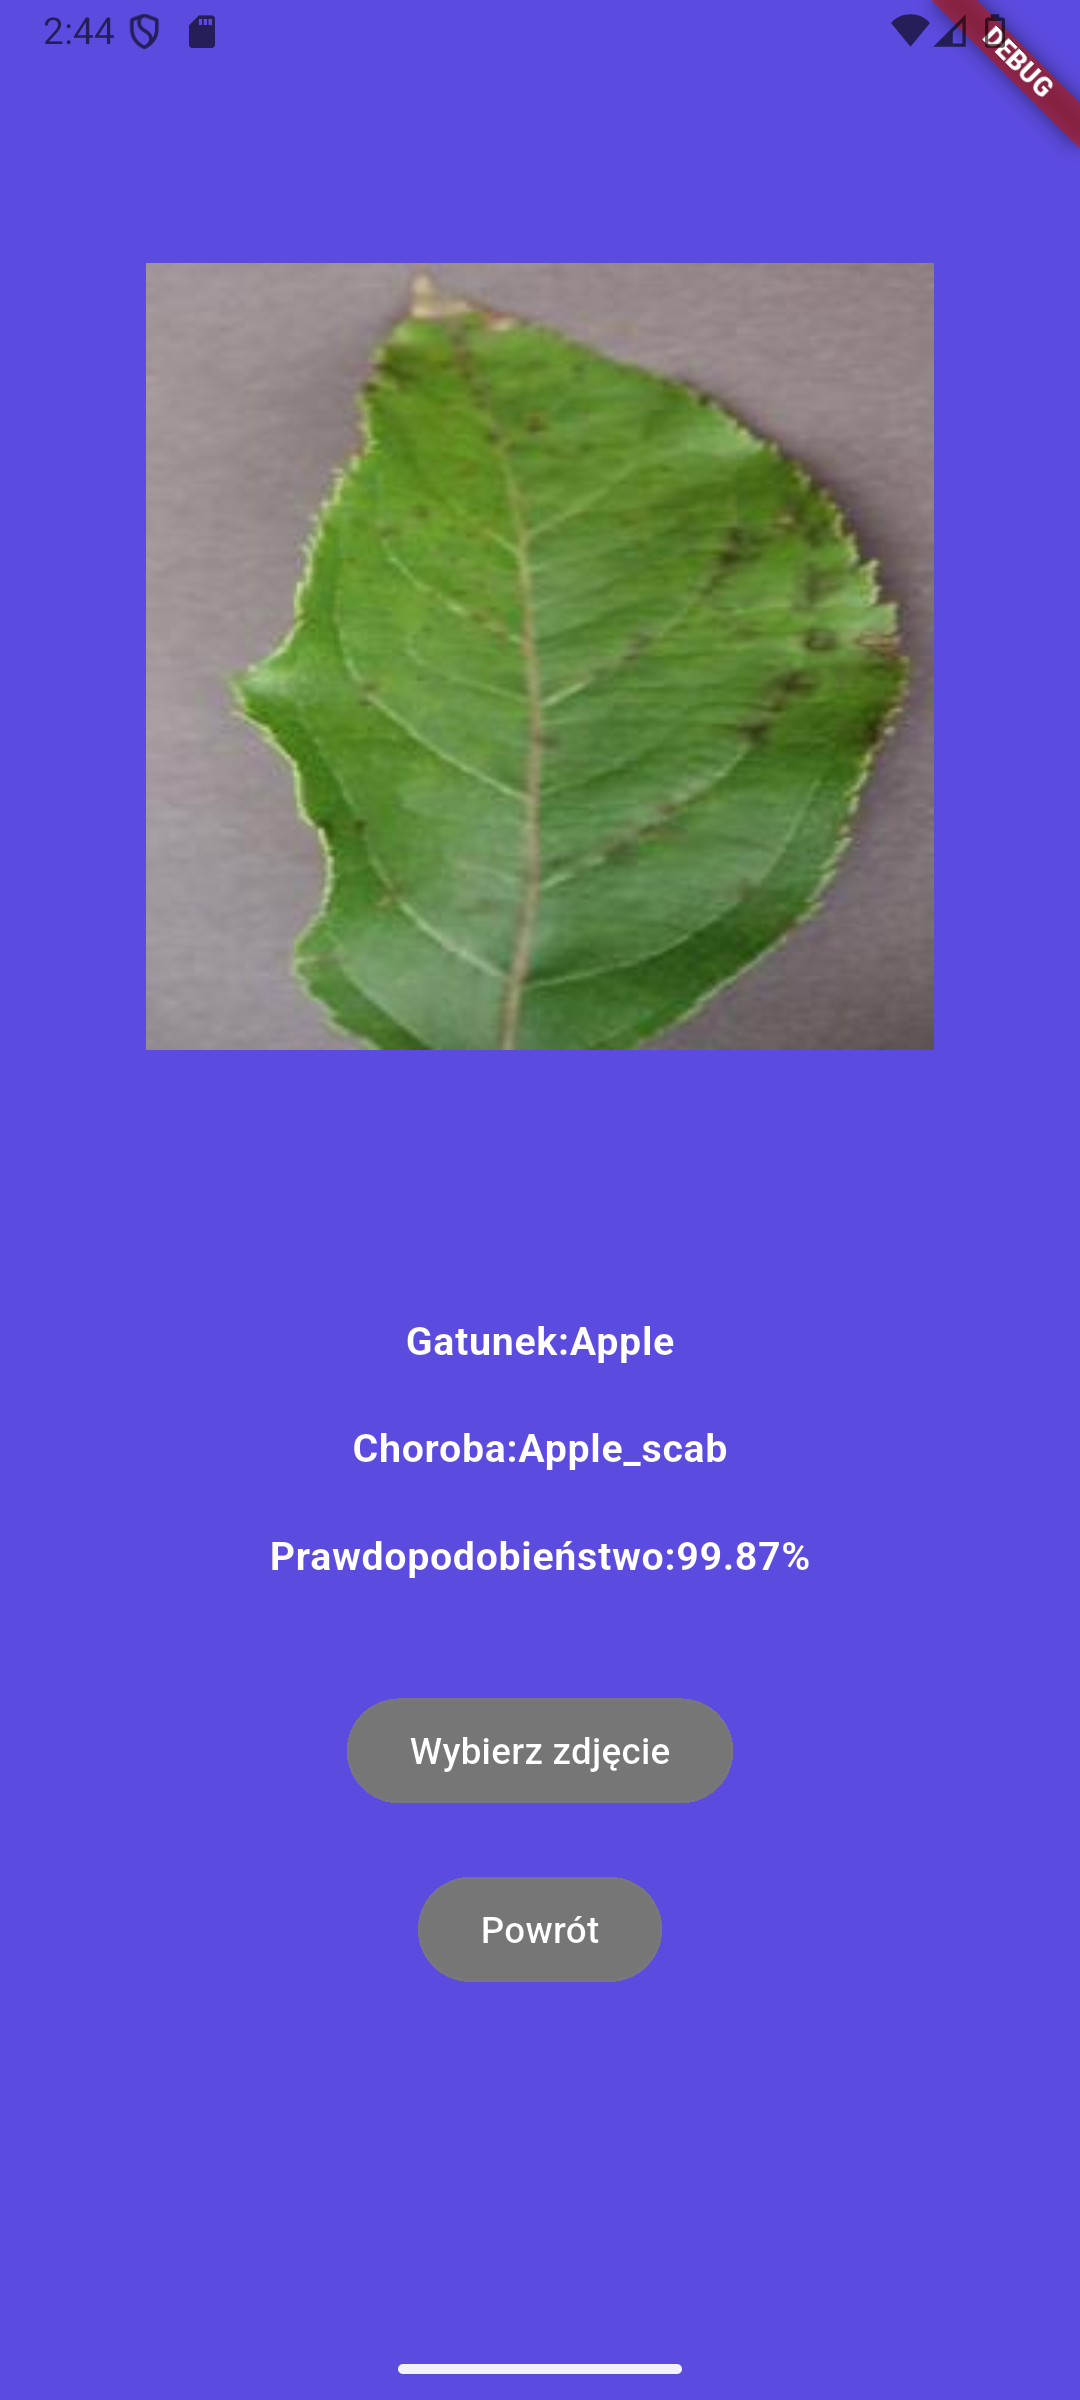
\includegraphics[width=0.3\textwidth]{img/aplikacja-2.png}
	\caption{Zdjęcie ekranu startowego oraz ekranu z wynikami }
	\label{fig:menu}
\end{figure}

W ramach pierwszego widoku aplikacja pozwala użytkownikowi na kliknięcie przycisku \textit{Wybierz zdjęcie}. Spowoduje to otwarcie galerii, gdzie użytkownik może wybrać zdjęcie przeznaczone do klasyfikacji.


W ramach widoku drugiego aplikacja wyświetla wyniki klasyfikacji uzyskane przez model oraz wybrane wcześniej zdjęcie. Użytkownik otrzymuje informację o gatunku rośliny, rozpoznanej chorobie oraz wartości prawdopodobieństwa poprawnie wykonanej klasyfikacji.

 Na tym ekranie znajdują się też dwa przyciski - \textit{Wybierz zdjęcie} oraz \textit{Powrót}. Kliknięcie pierwszego przycisku spowoduje ponowny wybór zdjęcia oraz ponowne wyświetlenie, już nowych, wyników. Drugi przycisk pozwala na powrót do ekranu startowego aplikacji.




\newpage
\section{Podsumowanie}
Celem pracy było zbadanie, jak wybrane architektury głębokiego uczenia różnią się pod względem skuteczności oraz odporności na redukcję liczby danych treningowych i degradację ich jakości w zadaniu klasyfikacji chorób roślin. Dodatkowym celem było stworzenie prototypu, w postaci aplikacji mobilnej, która jest przykładem wykorzystania badanego zagadnienia.

W ramach pracy przeprowadzono przegląd literatury,dokonano wyboru zbiór danych oraz przeglądu różnych technik uczenia maszynowego oraz przedstawiono wybrane architektury poddanych analizie - ViT, EfficientNet, MobileNet,  ResNet, oraz DenseNet. Przeprowadzono szereg eksperymentów pozwalających ocenić wpływ jakości oraz ilości danych na skuteczność badanych modeli. Uzyskane wyniki zostały wykorzystane w ramach analizy porównawczej architektur oraz umożliwiły określenie różnic w ich odporności na ograniczenia związane z ilością i jakością danych treningowych.  

 Na podstawie przeprowadzonych badań można stwierdzić, że większość analizowanych architektur biorących udział w badaniu jest skuteczna w ramach zadania klasyfikacji chorób roślin. Jedynym wyjątkiem jest  rodzina modeli DenseNet, gdzie oba warianty osiągnęły znacznie gorsze wyniki od pozostałych badanych modeli w obu przeprowadzonych eksperymentach. 
 
 Na podstawie pierwszego eksperymentu ustalono, największą odporność na zmniejszanie liczby danych treningowe mają modele MobileNetV2, EfficientNetB0 oraz EfficientNetB1. Miały one najmniejszą różnicę miary Macro F1. Najlepszy wynik dla całego zbioru uzyskały modele ResNet, jednak miały one większe spadki jakości, niż wcześniej wspomniane modele. Najlepszym kompromisem między jakością klasyfikacji, odpornością na spadek liczby danych oraz wymaganiami pamięciowymi stanowiły modele z rodziny MobileNet, które osiągały zbliżone wyniki do modeli z większą ilością parametrów, a przy tym nie odbiegały jakością od innych analizowanych modeli.
 
 Na podstawie drugiego eksperymentu ustalono, że największą odporność na zniekształcone dane treningowe mają modele ResNet50 oraz EfficientNetB1. Różnica między Macro F1 dla użytych zbiorów treningowych była dla nich najmniejsza i wynosiła zaledwie kilka tysięcznych. Najlepszym kompromisem, między jakością klasyfikacji, odpornością na spadek jakości danych oraz rozmiarem były modele z rodzin EfficientNet i MobileNet - ich wyniki były zbliżone do innych z zestawienia, a jednocześnie miały one zdecydowanie mniej parametrów.
 
 W ramach finalnej analizy obu eksperymentów ustalono, że najlepszym kompromisem między wynikami obu eksperymentów, a wydajnością pamięciową są rodziny EfficientNet i MobileNet. Najlepsze wyniki osiągały modele z rodziny ResNet, a najgorzej z oboma zadaniami radziły sobie modele z rodziny DenseNet. Nie zaobserwowano przewagi modeli opartych na transformerach nad modelami CNN - modele z rodziny ViT osiągały zbliżone, choć gorsze wyniki od modeli CNN. W ramach badania nie zaobserwowano także zależnosci między rozmiarem modelu a wynikami. Największe modele, z rodziny ViT, nie uzyskały przewagi nad modelami mniejszymi, a uzyskały wyniki gorsze. 
 
 
 \subsection{Dalsze kierunki badań}
 Otrzymane rezultaty badań stanowią podstawę do dalszych badań nad doborem i optymalizacją architektur przedstawionych w badaniu. Poprzez zastosowanie identycznych parametrów podczas trenowania modeli uzyskano wyniki, które można ze sobą obiektywnie porównać, wybrane hiperparametry mogą nie być optymalne dla danych modeli. Interesującym kierunkiem byłoby sprawdzenie, czy odpowiednie dobranie hiperparametrów i zastosowanie dodatkowych technik augmentacji danych pozwoliłoby uzyskać przewagę modelowi ViT nad CNN. W przyszłych badaniach warto także zastosować inny zbiór danych - dane wykorzystane w tym badaniu są zebrane w jednym, kontrolowanym środowisku laboratoryjnym. Sprawdzenie, czy modele radzą sobie w detekcji chorób \newline w środowisku naturalnym, gdzie zdjęcia mogą być wykonane pod różnym kątem, z różnym tłem, czy obiektami zasłaniającymi część liści pozwoliłoby ocenić, czy  dane modele są \newline w stanie znaleźć zastosowanie w warunkach rzeczywistych, bezpośrednio w gospodarstwie rolnym, a nie w kontrolowanym środowisku laboratoryjnym.  Dalsze badania mogłyby także rozszerzyć zakres badanych modeli - badanie to obejmowało tylko 10 modeli, \newline a analiza większej liczby architektur, w tym tych opartych o transformery, pozwoliłaby na szerszą ocenę oraz sprawdzenie, czy przewaga modeli CNN nad ViT utrzymuje się również w przypadku innych rozwiązań.
  
 



\newpage 
%--------------------------------------------
% Literatura
%--------------------------------------------
\cleardoublepage 
\printbibliography

%--------------------------------------------
% Spisy (opcjonalne)
%--------------------------------------------
\newpage
\pagestyle{plain}

% Wykaz symboli i skrótów.
% Pamiętaj, żeby posortować symbole alfabetycznie
% we własnym zakresie. Ponieważ mało kto używa takiego wykazu,
% uznałem, że robienie automatycznie sortowanej listy
% na poziomie LaTeXa to za duży overkill.
% Makro \acronymlist generuje właściwy tytuł sekcji,
% w zależności od języka.
% Makro \acronym dodaje skrót/symbol do listy,
% zapewniając podstawowe formatowanie.
% //AB
\vspace{0.8cm}
\acronymlist
\acronym{EiTI}{Wydział Elektroniki i Technik Informacyjnych}
\acronym{PW}{Politechnika Warszawska}
\acronym{WEIRD}{ang. \emph{Western, Educated, Industrialized, Rich and Democratic}}

\listoffigurestoc     % Spis rysunków.
\vspace{1cm}          % vertical space
\listoftablestoc      % Spis tabel.
\vspace{1cm}          % vertical space
\listofappendicestoc  % Spis załączników

% Załączniki
%\newpage
\appendix{Link do repozytorium GitHub}
%\lipsum[1-8]

%\newpage
%\appendix{Nazwa załącznika 2}
%\lipsum[1-4]

% Używając powyższych spisów jako szablonu,
% możesz tu dodać swój własny wykaz bądź listę,
% np. spis algorytmów.

\end{document}
